% !TeX root = ../index.tex
\chapter{Forms}
\graphicspath{{3-forms/images/}}

\section{Exercise 1}

\url{https://intweb.bucks.ac.uk/~21606555/oos/3-forms/ex1.html}
\captionsetup{type=figure}\captionof{figure}{ex1.html}
\subfile{pyg/src/3-forms/ex1}

\clearpage
\captionsetup{type=figure}\captionof{figure}{ex1-action.php}
\subfile{pyg/src/3-forms/ex1-action}

\begin{figure}[H]
  \caption{Input form for exercise 1}
  \centering
  \includegraphics[width=\textwidth]{ex1-form}
\end{figure}

\begin{figure}[H]
  \caption{Output of exercise 1}
  \centering
  \includegraphics[width=\textwidth]{ex1-result}
\end{figure}

\clearpage
\section{Exercise 2}

\url{https://intweb.bucks.ac.uk/~21606555/oos/3-forms/ex2.html}
\captionsetup{type=figure}\captionof{figure}{ex2.html}
\subfile{pyg/src/3-forms/ex2}

\captionsetup{type=figure}\captionof{figure}{ex2-action.php}
\subfile{pyg/src/3-forms/ex2-action}

\begin{figure}[H]
  \caption{Input form for exercise 2 showing male/under 21}
  \centering
  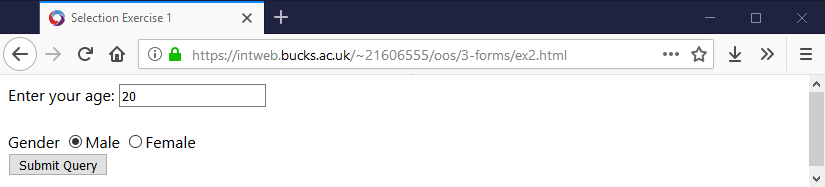
\includegraphics[width=\textwidth]{ex2-male-form}
\end{figure}

\begin{figure}[H]
  \caption{Output of exercise 2 showing male/under 21}
  \centering
  
\includegraphics[width=\textwidth]{ex2-male-result}
\end{figure}

\begin{figure}[H]
  \caption{Input form for exercise 2 showing female/over 21}
  \centering
  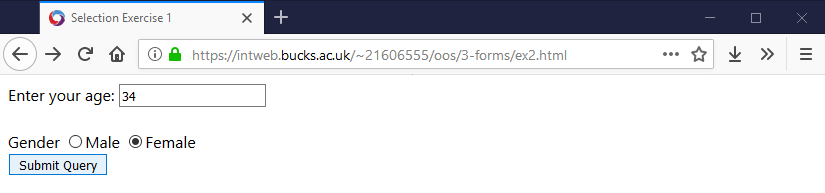
\includegraphics[width=\textwidth]{ex2-female-form}
\end{figure}

\begin{figure}[H]
  \caption{Output of exercise 2 showing female/over 21}
  \centering
  \includegraphics[width=\textwidth]{ex2-female-result}
\end{figure}

\clearpage
\section{Exercise 3}

If all the breaks are removed from the switch statement then the correct case is still accessed (selecting Part Time prints the part time course and not HNC, HND or BSC). However it will also print the default switch case (no course selected).\\

This happens as the \texttt{break} keyword is used to exit the switch statement. If there is no break then it will keep going through the switch cases for anything else that matches - the default case matches anything.\\

\url{https://intweb.bucks.ac.uk/~21606555/oos/3-forms/ex3.html}

\captionsetup{type=figure}\captionof{figure}{ex3.html}
\subfile{pyg/src/3-forms/ex3}

\captionsetup{type=figure}\captionof{figure}{ex3-action.php}
\subfile{pyg/src/3-forms/ex3-action}

\begin{figure}[H]
  \caption{Input form for exercise 3}
  \centering
  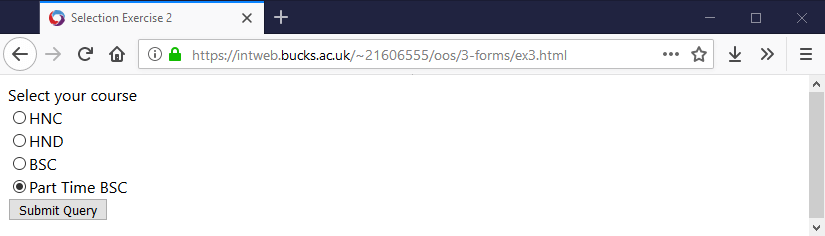
\includegraphics[width=\textwidth]{ex3-form}
\end{figure}

\begin{figure}[H]
  \caption{Output of exercise 3}
  \centering
  \includegraphics[width=\textwidth]{ex3-result}
\end{figure}

\clearpage
\section{Exercise 4}

\url{https://intweb.bucks.ac.uk/~21606555/oos/3-forms/ex4.php}
\captionsetup{type=figure}\captionof{figure}{ex4.php}
\subfile{pyg/src/3-forms/ex4}

\begin{figure}[H]
  \caption{Input form for exercise 4}
  \centering
  \includegraphics[width=\textwidth]{ex4-form}
\end{figure}

\begin{figure}[H]
  \caption{Output of exercise 4}
  \centering
  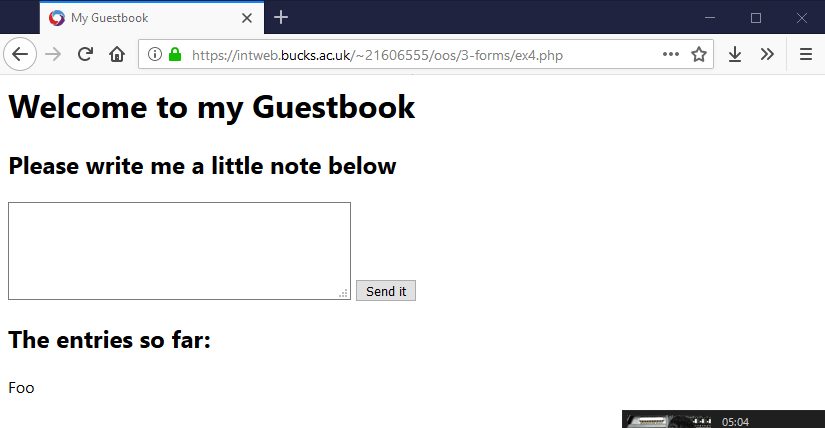
\includegraphics[width=\textwidth]{ex4-result}
\end{figure}
